\begin{figure}[htbp]
    \centering
    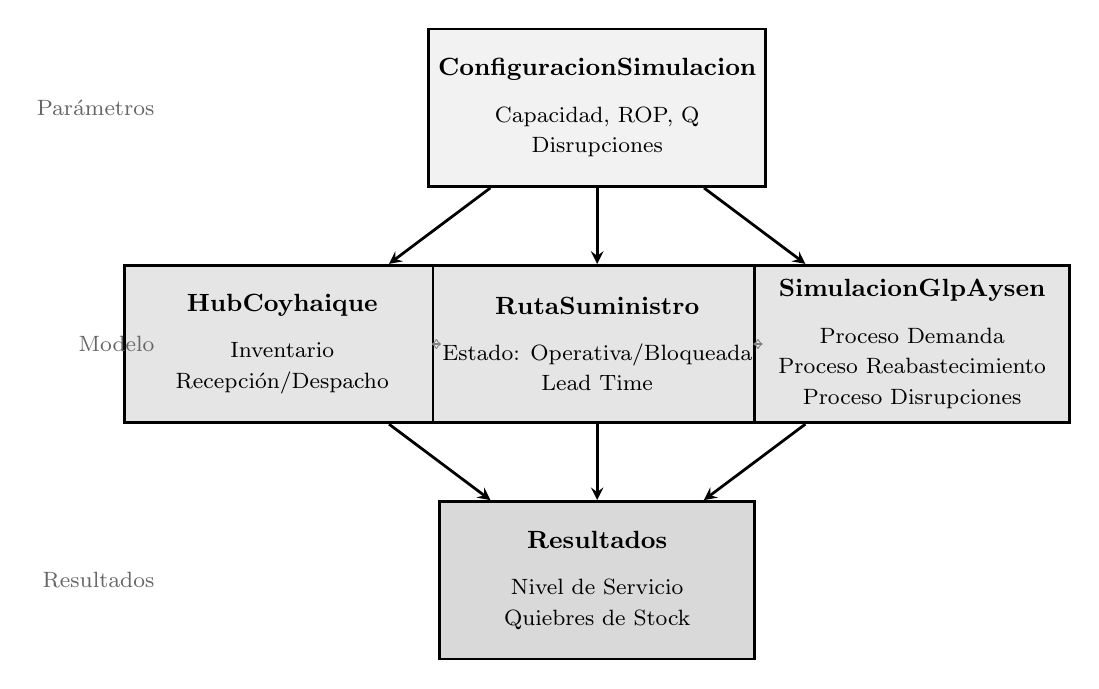
\begin{tikzpicture}[
        font=\small,
        node distance=1.5cm,
        box/.style={
            rectangle, draw=black, line width=1pt,
            minimum height=2cm, minimum width=4cm,
            text centered, font=\small, align=center
        },
        arrow/.style={->, >=stealth, line width=1pt}
    ]

        % Capa 1: Configuración
        \node[box, fill=gray!10] (config) at (0,6) {
            \textbf{ConfiguracionSimulacion}\\[0.2cm]
            \footnotesize Capacidad, ROP, Q\\
            \footnotesize Disrupciones
        };

        % Capa 2: Modelo
        \node[box, fill=gray!20] (hub) at (-4,3) {
            \textbf{HubCoyhaique}\\[0.2cm]
            \footnotesize Inventario\\
            \footnotesize Recepción/Despacho
        };

        \node[box, fill=gray!20] (ruta) at (0,3) {
            \textbf{RutaSuministro}\\[0.2cm]
            \footnotesize Estado: Operativa/Bloqueada\\
            \footnotesize Lead Time
        };

        \node[box, fill=gray!20] (sim) at (4,3) {
            \textbf{SimulacionGlpAysen}\\[0.2cm]
            \footnotesize Proceso Demanda\\
            \footnotesize Proceso Reabastecimiento\\
            \footnotesize Proceso Disrupciones
        };

        % Capa 3: Métricas
        \node[box, fill=gray!30] (metricas) at (0,0) {
            \textbf{Resultados}\\[0.2cm]
            \footnotesize Nivel de Servicio\\
            \footnotesize Quiebres de Stock
        };

        % Flechas verticales
        \draw[arrow] (config) -- (hub);
        \draw[arrow] (config) -- (ruta);
        \draw[arrow] (config) -- (sim);

        \draw[arrow] (hub) -- (metricas);
        \draw[arrow] (ruta) -- (metricas);
        \draw[arrow] (sim) -- (metricas);

        % Interacción entre componentes
        \draw[<->, dashed, gray] (hub.east) -- (ruta.west);
        \draw[<->, dashed, gray] (ruta.east) -- (sim.west);

        % Etiquetas de capas
        \node[anchor=east, font=\footnotesize, color=black!60] at (-5.5,6) {Parámetros};
        \node[anchor=east, font=\footnotesize, color=black!60] at (-5.5,3) {Modelo};
        \node[anchor=east, font=\footnotesize, color=black!60] at (-5.5,0) {Resultados};

    \end{tikzpicture}
    \caption{Arquitectura modular del sistema de simulación en tres capas.}
    \label{fig:arquitectura-software}
\end{figure}
